%%%%%%%%%%%%%%%%%%%%%%%%%%%%%%%%%%%%%%%%%%%%
\section{Talleres}

\begin{frame}
      \frametitle{Contenido}
      \tableofcontents[currentsection]
\end{frame}


%%%%%%%%%%%%%%%%%%%%%%%%%%%%%%%%%%%%%%%%%%%%%
\subsection{
Curriculum de cuatro lecciones
}

%%%%%%%%%%%%%%%%%%%%%%%%%%%%%%%%%%%%%%%%%%%%%%%%%%%%%%%%
{
\paper{Badillo-Perez A, Badillo-Perez D, Barco A, Montenegro R, Xochicale M. 2013, Teaching AI and Robotics to Children in a Mexican town, DEI-HRI2023, \url{https://arxiv.org/abs/2303.03956}}

\begin{frame}{Curriculum}
      \begin{figure}
        \centering
        \includegraphics[width=1.0\textwidth]{./curriculum/outputs/drawing-v00.png}
        %\caption{}
      \end{figure}
\end{frame}
}


%%%%%%%%%%%%%%%%%%%%%%%%%%%%%%%%%%%%%%%%%%%%%
\subsection{
Piloteando el curriculum
}

%%%%%%%%%%%%%%%%%%%%%%%%%%%%%%%%%%%%%%%%%%%%%%%%%%%%%%%%
{
\paper{Badillo-Perez A, Badillo-Perez D, Barco A, Montenegro R, \textbf{Xochicale M. 2023}, Teaching AI and Robotics to Children in a Mexican town, DEI-HRI2023, \url{https://arxiv.org/abs/2303.03956}}

\begin{frame}{Participantes}

\begin{itemize}
\item 14 participantes de los cuales 10 atendieron el taller, 6 hombres y 4 mujeres (de edad en a\~nos: promedio=8 and desviaci\'on estandar=$\pm$1.61)     
\item 4 instructores con diferentes niveles de experiencia en ense\~nanza a ni\~nos y jovenes.
\end{itemize}

\end{frame}
}




%%%%%%%%%%%%%%%%%%%%%%%%%%%%%%%%%%%%%%%%%%%%%%%%%%%%%%%%
{
\paper{Badillo-Perez A, Badillo-Perez D, Barco A, Montenegro R, \textbf{Xochicale M. 2023}, Teaching AI and Robotics to Children in a Mexican town, DEI-HRI2023, \url{https://arxiv.org/abs/2303.03956}}

\begin{frame}{
%Piloting workshop: Coding and bingo activities
Piloteando talleres: Codificando y el juego de bingo
}
      \begin{figure}
        \centering
        \includegraphics[width=1.0\textwidth]{./pilot-workshop-a/outputs/drawing-v00.png}
        %\caption{}
      \end{figure}
\end{frame}
}



%%%%%%%%%%%%%%%%%%%%%%%%%%%%%%%%%%%%%%%%%%%%%%%%%%%%%%%%
{

\paper{Badillo-Perez A, Badillo-Perez D, Barco A, Montenegro R, \textbf{Xochicale M. 2023}, Teaching AI and Robotics to Children in a Mexican town, DEI-HRI2023, \url{https://arxiv.org/abs/2303.03956}}

\begin{frame}{
%Piloting workshop: Teaching activities
Piloteando talleres: Actividades de ense\~nanza
}
      \begin{figure}
        \centering
        \includegraphics[width=1.0\textwidth]{./pilot-workshop-b/outputs/drawing-v00.png}
        %\caption{}
      \end{figure}
\end{frame}
}

%%%%%%%%%%%%%%%%%%%%%%%%%%%%%%%%%%%%%%%%%%%%%%%%%%%%%%%%
{

\paper{Badillo-Perez A, Badillo-Perez D, Barco A, Montenegro R, \textbf{Xochicale M. 2023}, Teaching AI and Robotics to Children in a Mexican town, DEI-HRI2023, \url{https://arxiv.org/abs/2303.03956}}

\begin{frame}{
%Piloting workshop: Group activities
Piloteando talleres: Actividades en grupo
}
      \begin{figure}
        \centering
        \includegraphics[width=1.0\textwidth]{./pilot-workshop-c/outputs/drawing-v00.png}
        %\caption{}
      \end{figure}
\end{frame}
}

%%%%%%%%%%%%%%%%%%%%%%%%%%%%%%%%%%%%%%%%%%%%%
\subsection{
%Results of the survey
Resultados de las encuestas
}

%%%%%%%%%%%%%%%%%%%%%%%%%%%%%%%%%%%%%%%%%%%%%%%%%%%%%%%%
{

\paper{Badillo-Perez A, Badillo-Perez D, Barco A, Montenegro R, \textbf{Xochicale M. 2023}, Teaching AI and Robotics to Children in a Mexican town, DEI-HRI2023, \url{https://arxiv.org/abs/2303.03956}}

\begin{frame}{
%Survey results
Resultados de las encuestas
}
      \begin{figure}
        \centering
        \includegraphics[width=1.0\textwidth]{./survey-results/outputs/drawing-v00.png}
        %\caption{}
      \end{figure}
\end{frame}
}



%%%%%%%%%%%%%%%%%%%%%%%%%%%%%%%%%%%%%%%%%%%%%%%%%%%%%%%%
{
\paper{Badillo-Perez A, Badillo-Perez D, Barco A, Montenegro R, \textbf{Xochicale M. 2023}, Teaching AI and Robotics to Children in a Mexican town, DEI-HRI2023, \url{https://arxiv.org/abs/2303.03956}}

\begin{frame}{An\'alisis estad\'istico}

\begin{itemize}
%\item A Wilcoxon T test was used to analyze the results of the survey before and after the survey to see if the engineering attitudes had a significant effect on pre and post survey of the workshop.
\item Prueba Wilcoxon T se uso para analizar los resultados de las encuentas antes y despu\'es para probar si las actitudes de ingenierian tuvieron un efecto significativo.
%\item The average survey before the test was lower ($\mu$ = 2.194500 $\pm \sigma$ 0.558367 ) compared to the posttest results ($\mu$ = 2.239500 $\pm \sigma$= 0.396796).
\item El promedio de la prueba antes de la encuesta es menor ($\mu$ = 2.194500 $\pm \sigma$ 0.558367 ) comparado a la prueba despu\'es de la encuesta ($\mu$ = 2.239500 $\pm \sigma$= 0.396796).
%\item There was no statistically significant in the increase of attitudes towards engineering (t=53.5, p= 0.45).
\item Los resultados no muestra un resultado estadisticamente significativo en el incremento de la atidudes hacia ingenier\'ia y ciencia (t=53.5, p= 0.45).
\end{itemize}

%See Appendix section for reproducible Jupyter notebooks of statistical analysis and plots.
Ver el apendice con codigo en Jupyter para su replicaci\'on.

\end{frame}
}

